\chapter{Abstract Stack Machine}

The notion of \emph{abstract machine} is a convenient concept in the field of programming languages, compliers and tools.
As the name suggests, abstract machine is a hypothetical computational device which fills the gap between a high-level language
and an actual hardware. It, therefore, introduces an additional intermediate abstraction level which facilitates the
decomposition of many compiler implementation and program analysis tasks. This decomposition makes it possible to separate
certain implementation subtasks, solve them and assess the correctness of solutions independently.

An important question is how an abstract machine can be specified and built. Do we need a blueprint, what appliances and equipment
should we use for its manufacturing? Fortunately, it turns out that we already have all what we need in our toolbox. For us an
abstract machine is just a language, and to specify an abstract machine we need to specify the syntax and semantics of
this language. Implementing an abstract machine amounts to implementing its interpreter. In this section we
give the syntax and semantics of a \lama-specific abstract stack machine, describe the compiler from straight-line
programs language into this abstract machine and prove its correctness. But, first, we briefly survey the variety of existing
flavours of abstract machines and discuss the motivation for the basic features of that we chose.

\section{The Variety of Abstract Machines}

Abstract machines share a lot of common features with actual hardware. They are programmable devices, and their
programs consist of instructions each of which is capable of performing a rather simple operation. On the other hand,
abstract machines often provide a direct way of representing and using \emph{meta-information} specific to a certain
lanaguage or a group of languages this abstract machine is devised to support. This may include types, object structures, etc.
For example, JVM directly supports such construct as virtual method call, which for a real hardware has to be
implemented using the knowledge of actual virtual methods table layout, etc. 



\begin{figure}[t]
  \centering

  \begin{subfigure}[t]{\textwidth}
   \centering
    $x*y+3$
    \caption{Expression}
    \label{expr}
  \end{subfigure}
  \vskip5mm
  \begin{subfigure}[t]{0.3\textwidth}
  \begin{verbatim}
      LD x
      LD y
      MUL
      CONST 3
      ADD
  \end{verbatim}  
  \caption{Stack Machine Code}
  \label{expr-stack}
  \end{subfigure}
  \begin{subfigure}[t]{0.3\textwidth}
  \begin{verbatim}
      MUL x, y, %1
      ADD %1, 3, %2


      
  \end{verbatim}  
  \caption{Three-address Code}
  \label{expr-3addr}
  \end{subfigure}
  \begin{subfigure}[t]{0.3\textwidth}
  \begin{verbatim}
      MOV y, %1
      MUL x, %1
      ADD 3, %1

      
  \end{verbatim}  
  \caption{Two-address Code}
  \label{expr-2addr}
  \end{subfigure}
  \caption{An Expression and Its Abstract Machine Code}
\end{figure}

There are different flavours of abstract machines. For now, as we are dealing with rather a simple language of
straight-line programs, only one essential feature is important: the representation of \emph{temporaries}.

In our language (and the majority of conventional programming languages) expressions can contain an arbitrary
number of operators. However, actual hardware (and the majority of abstract machines) cannot evaluate arbitrarily
large expressions ``in one step''. It evaluates them operator by operator, storing somewhere intermediate results, otherwise
called \emph{temporary values}. There are two major disciplines to work with temporaries:

\begin{itemize}
\item Using a \emph{stack}. With this discipline all temporary values are stored on a stack specifically disignated
  for this purpose. Thus, all operators take the operands from the stack and put the result back. This, in particular,
  means that the majority of instructions do not have explicit operands.
  
\item Using a potentially infinite number of named locations (often called \emph{pseudo-registers}). Under this approach
  the operands of each instruction (if any) are explicitly annotated. There are two commonly used special cases: \emph{three-address code},
  when an instruction can have up to three distinct operands (two for arguments and one for the result) and
  \emph{two-address code}, when an instruction can have no more than two operands, one of which serves simultaneously
  as an argument and as the result.
\end{itemize}

All these versions of abstract machines have their merits and shortcomings, and rather easier to switch to and from. Stack code is known
to be very compact (indeed, it does not require extra space to specify the operands for the majority of instructions); it is also a
little bit easier to generate. As the same time code with explicit operands is easier to analyize and transform, and faster to
interpret. It worth mentioning that the distinction stack vs. explicit operands by no means separates abstract machines from
real hardware: there some examples of the latter which implement stack architecture (the most notable, probably, is now late
Intel 8087 floating-point coprocessor).

In our case we favoured stack machine over others since the compilation to stack code posesses some nice invariants and
its correctness can be formally assessed easily. In addition the archiecture of \textsc{x86} is very close to two-address
code, so dealing with stack abstract machine allows us to consider a broader class of architectures.

\section{Syntax and Semantics}

The syntax of abstract stack machine language is shown below:

\[
\begin{array}{rcl}
  \mathscr{I} & = & \llang{BINOP$\;\otimes$}\\
              &   & \llang{CONST $\;\mathbb{N}$}\\
              &   & \llang{LD$\;\mathscr{X}$}\\
              &   & \llang{ST$\;\mathscr{X}$}\\
              &   & \llang{READ}\\
              &   & \llang{WRITE}\\[2mm]
  \mathscr{S} & = & \epsilon\\
              &   & \mathscr{I}\mathscr{S}
\end{array}
\]

We have here two syntactic categories~--- \emph{instructions} $\mathscr{I}$ and \emph{programs} $\mathscr{P}$.

There are six types of instructions, and only two types of programs~--- an empty program $\epsilon$ and a composite
program which consists of an instruction and a residual program. In essence the programs of stack machine
are just lists of instructions. Some of instructions have operands: for \llang{BINOP} an operand is a name of binary operator
from the source language, for \llang{CONST} it is a natural number, for \llang{LD} and \llang{ST}~--- the names of
variables. We can notice that the language of stack machine is very simple, much simpler than that for the straight-line programs. Yet it
possesses enough expressive power to perform the same calculations as an arbitrary straigh-line program! We assess this property
by implementing a compiler and proving its correctness.

Before giving a formal semantics for stack machine we first give an informal description of how it functions. The stack
machine operates in a similar environment as straight-line programs. It reads and writes numbers from/to a world, and it
posesses an internal state which binds (some) variables names to integer values. Beside that, stack machine has a
stack of integers at its discretion. In a nutshell, this stack contains temporary values which are nowhere to place
otherwise. The stack machine program executes instruction by instruction starting from the first instruction.
Each instruction modifies the configuration of the stack machine (state, stack, or world) and can either succeed or
fail (crash). The machine stops when there are no instructions left to execute; in this case the contents of
the output stream is taken as the result of stack program evaluation.

\begin{figure}[t]
  \[
  \def\arraystretch{3}
  \arraycolsep=10pt
  \def\arraystretch{3}
  \begin{array}{cr} 
  \trans{c}{\epsilon}{c}&\ruleno{Stop$_{SM}$}\\
  \trule{\trans{\inbr{\sigma,\,(x\oplus y)s,\,\omega}}{p}{c^\prime}}{\trans{\inbr{\sigma,\,yxs,\,\omega}}{[\llang{BINOP $\;\otimes$}]p}{c^\prime}}&\ruleno{Binop$_{SM}$}\\
  \trule{\trans{\inbr{\sigma,\,zs,\,\omega}}{p}{c^\prime}}{\trans{\inbr{\sigma,\,s,\,\omega}}{[\llang{CONST $\;z$}]p}{c^\prime}}&\ruleno{Const$_{SM}$}\\
  \trule{\inbr{z,\,\omega^\prime}=\primi{read}{\;\omega},\,\trans{\inbr{\sigma,\,zs,\,\omega^\prime}}{p}{c^\prime}}{\trans{\inbr{\sigma,\,s,\,\omega}}{[\llang{READ}]\,p}{c^\prime}}&\ruleno{Read$_{SM}$}\\
  \trule{\trans{\inbr{\sigma,\,s,\,\primi{write}{\;z\;\omega}}}{p}{c^\prime}}{\trans{\inbr{\sigma,\,zs,\,\omega}}{[\llang{WRITE}]\,p}{c^\prime}}&\ruleno{Write$_{SM}$}\\
  \trule{\trans{\inbr{\sigma,\,(\sigma\;x)s,\,\omega}}{p}{c^\prime}}{\trans{\inbr{\sigma,\,s,\,\omega}}{[\llang{LD $\;x$}]p}{c^\prime}}&\ruleno{LD$_{SM}$}\\
  \trule{\trans{\inbr{\sigma\,[x\,gets z],\,s,\,\omega}}{p}{c^\prime}}{\trans{\inbr{\sigma,\,zs,\,\omega}}{[\llang{ST $\;x$}]p}{c^\prime}}&\ruleno{ST$_{SM}$}
  \end{array}
  \]
  \caption{Big-step operational semantics for stack machine}
  \label{sm-bigstep}
\end{figure}

We describe this behavior, again, using a big-step operational semantics. First, we define the extended configuration $\mathscr{C}_{\mathscr{SM}}$
for stack machine as

\[
\mathscr{C}_{\mathscr{SM}}=St\times\mathbb{Z}^*\times\mathscr{W}
\]

\setsubarrow{^\ph_{\mathscr{SM}}}

Each component of extended configuration~--- state, stack of integers, word~--- is familiar to us. Next we need
to specify the big-step transition relation \mbox{``$\transrel$''} for stack machines. The rules of the semantics
are given in Fig.~\ref{sm-bigstep}. In the rules we additionaly surrounded the head instruction of a program
by square brackets \lstinline|[...]| to visually separate it from the rest of the program.

The first rule, \rulename{Stop$_{SM}$}, is at the same time the single axiom in the semantics. It tells us that an empty
program does not change the configuration. This, in particular, happens when all instructions of a program were
already evaluated and there is nothing left to evaluate.

All other rules follow the same pattern: they describe the effect of the first instruction of the current program,
and then prescribe to evaluate the rest of the program using the same evluation relation.

Rule \rulename{Binop$_{SM}$} describes the case when the first instruction is a binary operator. To succeed, this instruction
requires atleast two integer values, $x$ and $y$, to reside on the stack. If so, it combines these values using binary
operator $\oplus$ and puts the result back on the stack. The correspondence between ``$\otimes$'' and ``$\oplus$'' is,
of course, the same as for the semantics of straght-line programs (see a table of the page~\pageref{times-plus-tab}).

Rule \rulename{Const$_{SM}$} corresponds to the case when the first instruction is \llang{CONST$\;z$}. This instruction
puts its operand $z$ on the stack.

The next two symmetrical rules, \rulename{Read$_{SM}$} and \rulename{Write$_{SM}$}, deal with instructions \llang{READ} and
\llang{WRITE} respectively. \llang{READ} reads a value from input stream and puts it on the stack; if the input stream is
empty the instruction fails. \llang{WRITE} takes a valus from the top of the stack and puts it in the output stream; this
instruction fails if the stack is empty.

Finally, two last rules, \rulename{LD$_{SM}$} and \rulename{ST$_{SM}$}, desribe the semantics of instructions \llang{LD} and
\llang{ST}. Both instructions have an operand, the name of a variable. \llang{LD$\;x$} puts the value of variable $x$, associated
in the current state $\sigma$, on the stack. It fails if $\sigma\;x$ is undefined. \llang{ST$\;x$} takes the top value from the
stack and updates the current state $\sigma$ to associate $x$ with this value. It fails if the stack is empty.

With the transition relation $\transrel$ defined we can specify the ``surface'' semantics for stack machine programs $\sembr{\bullet}^\ph_{\mathscr{SM}}$:

\[
  \begin{array}{c}
    \sembr{\bullet}^\ph_{SM} : \mathscr{S}\to \mathbb{Z}^*\to \mathbb{Z}^*\\[2mm]
      \trule{\trans{\inbr{\Lambda,\,\epsilon,\,\inbr{i,\,\epsilon}}}{p}{\inbr{\sigma,\,s,\,\omega}}}
            {\sembr{p}^\ph_{SM}\;i=\primi{out}{\;\omega}}
  \end{array}
\]

In other words, we take an input $i$, create an initial configuration, consisting of an empty state $\Lambda$, empty stack $\epsilon$ and an
initial world $\inbr{i,\,\epsilon}$, then run the program and, if it eventually comes to an end with some final configuration $\inbr{\sigma,\,s,\,\omega}$, we take
output stream from this configuration's world as the result of the evaluation.

As always, we can identify the following important properties of the semantics:

\begin{itemize}
\item \emph{Determinism:} for each program and each configuration there is at most one rule that can be applied; thus, if (for arbitrary $i$ and $p$)
  $\sembr{p}^\ph_{SM}\;i=o$ and   $\sembr{p}^\ph_{SM}\;i=o^\prime$ then $o=o^\prime$;
\item \emph{Compositionality}: the premise of each rule deals with programs one instruction shorter, than the conclusion. This, again, means that
  the principle of structural induction can be applied for proving the properties of the semantics.
\end{itemize}

It is also worth discussing the ``shape'' of derivation which the rules of the semantics generate. As we can see, each rule (except for the axiom) has
exactly one premise, and the final configuration of the primise is at the same time the final configuration of the conclusion. This means that
the derivations in this semantics have the form of a ``tower''; the top of the tower corresponds to the application of the single axiom, which
transfers its initial configuration to final one unchanged, and after that this final configuration is propagated down the tower in the right-hand side
configurations of all involved rules. The effects of individual instructions can be traced in the bottom-up manner in the left-hand side configurations of the
rules comprising the tower. To illustrate this structure, consider the following stack machine program:

\begin{verbatim}
   READ
   READ
   BINOP +
   WRITE
\end{verbatim}

The derivation ``tower'' which corresponds to the evaluation of this program for the input $\inbr{2,\,3}$ is shown in Fig.~\ref{derivation-tower}. As always,
we omit program for space considerations; the solid arrows connect the ``floors'' of the tower while dashed ones show the configurations' data flow.

\begin{figure}[t]
  \centering
  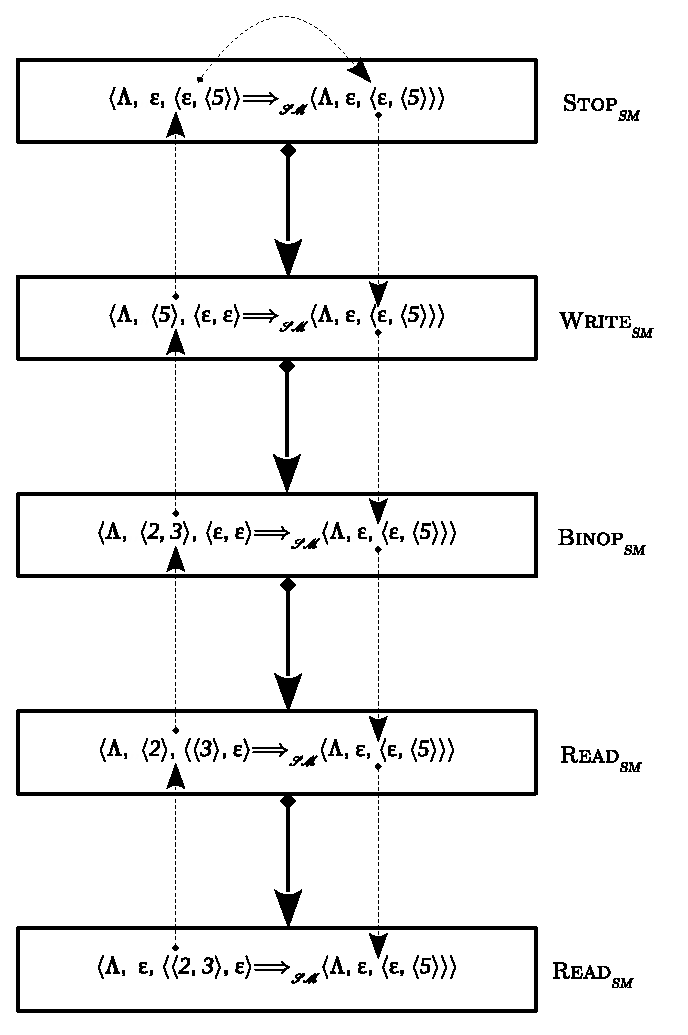
\includegraphics[scale=0.8]{images/05-01.eps}
  \caption{Derivation ``tower'' example}
  \label{derivation-tower}
\end{figure}

\section{Stack Machine Compiler}

In this section we describe a compiler from straigh-line programs language to the abstract stack machine and prove its correctness.
